% Created 2017-09-11 Mon 14:46
\documentclass[9pt,lineo]{elife}

\usepackage{amsmath}
\usepackage{amssymb}
\usepackage[version=4]{mhchem}
\usepackage{siunitx}


              \usepackage[utf8]{inputenc}
\sisetup{detect-all}
\setcounter{secnumdepth}{0}
\date{\today}
\title{}
\hypersetup{
 pdfauthor={},
 pdftitle={},
 pdfkeywords={},
 pdfsubject={},
 pdfcreator={Emacs 25.1.2 (Org mode 8.3.5)}, 
 pdflang={English}}
\begin{document}

\begin{figure}
\begin{fullwidth} \centering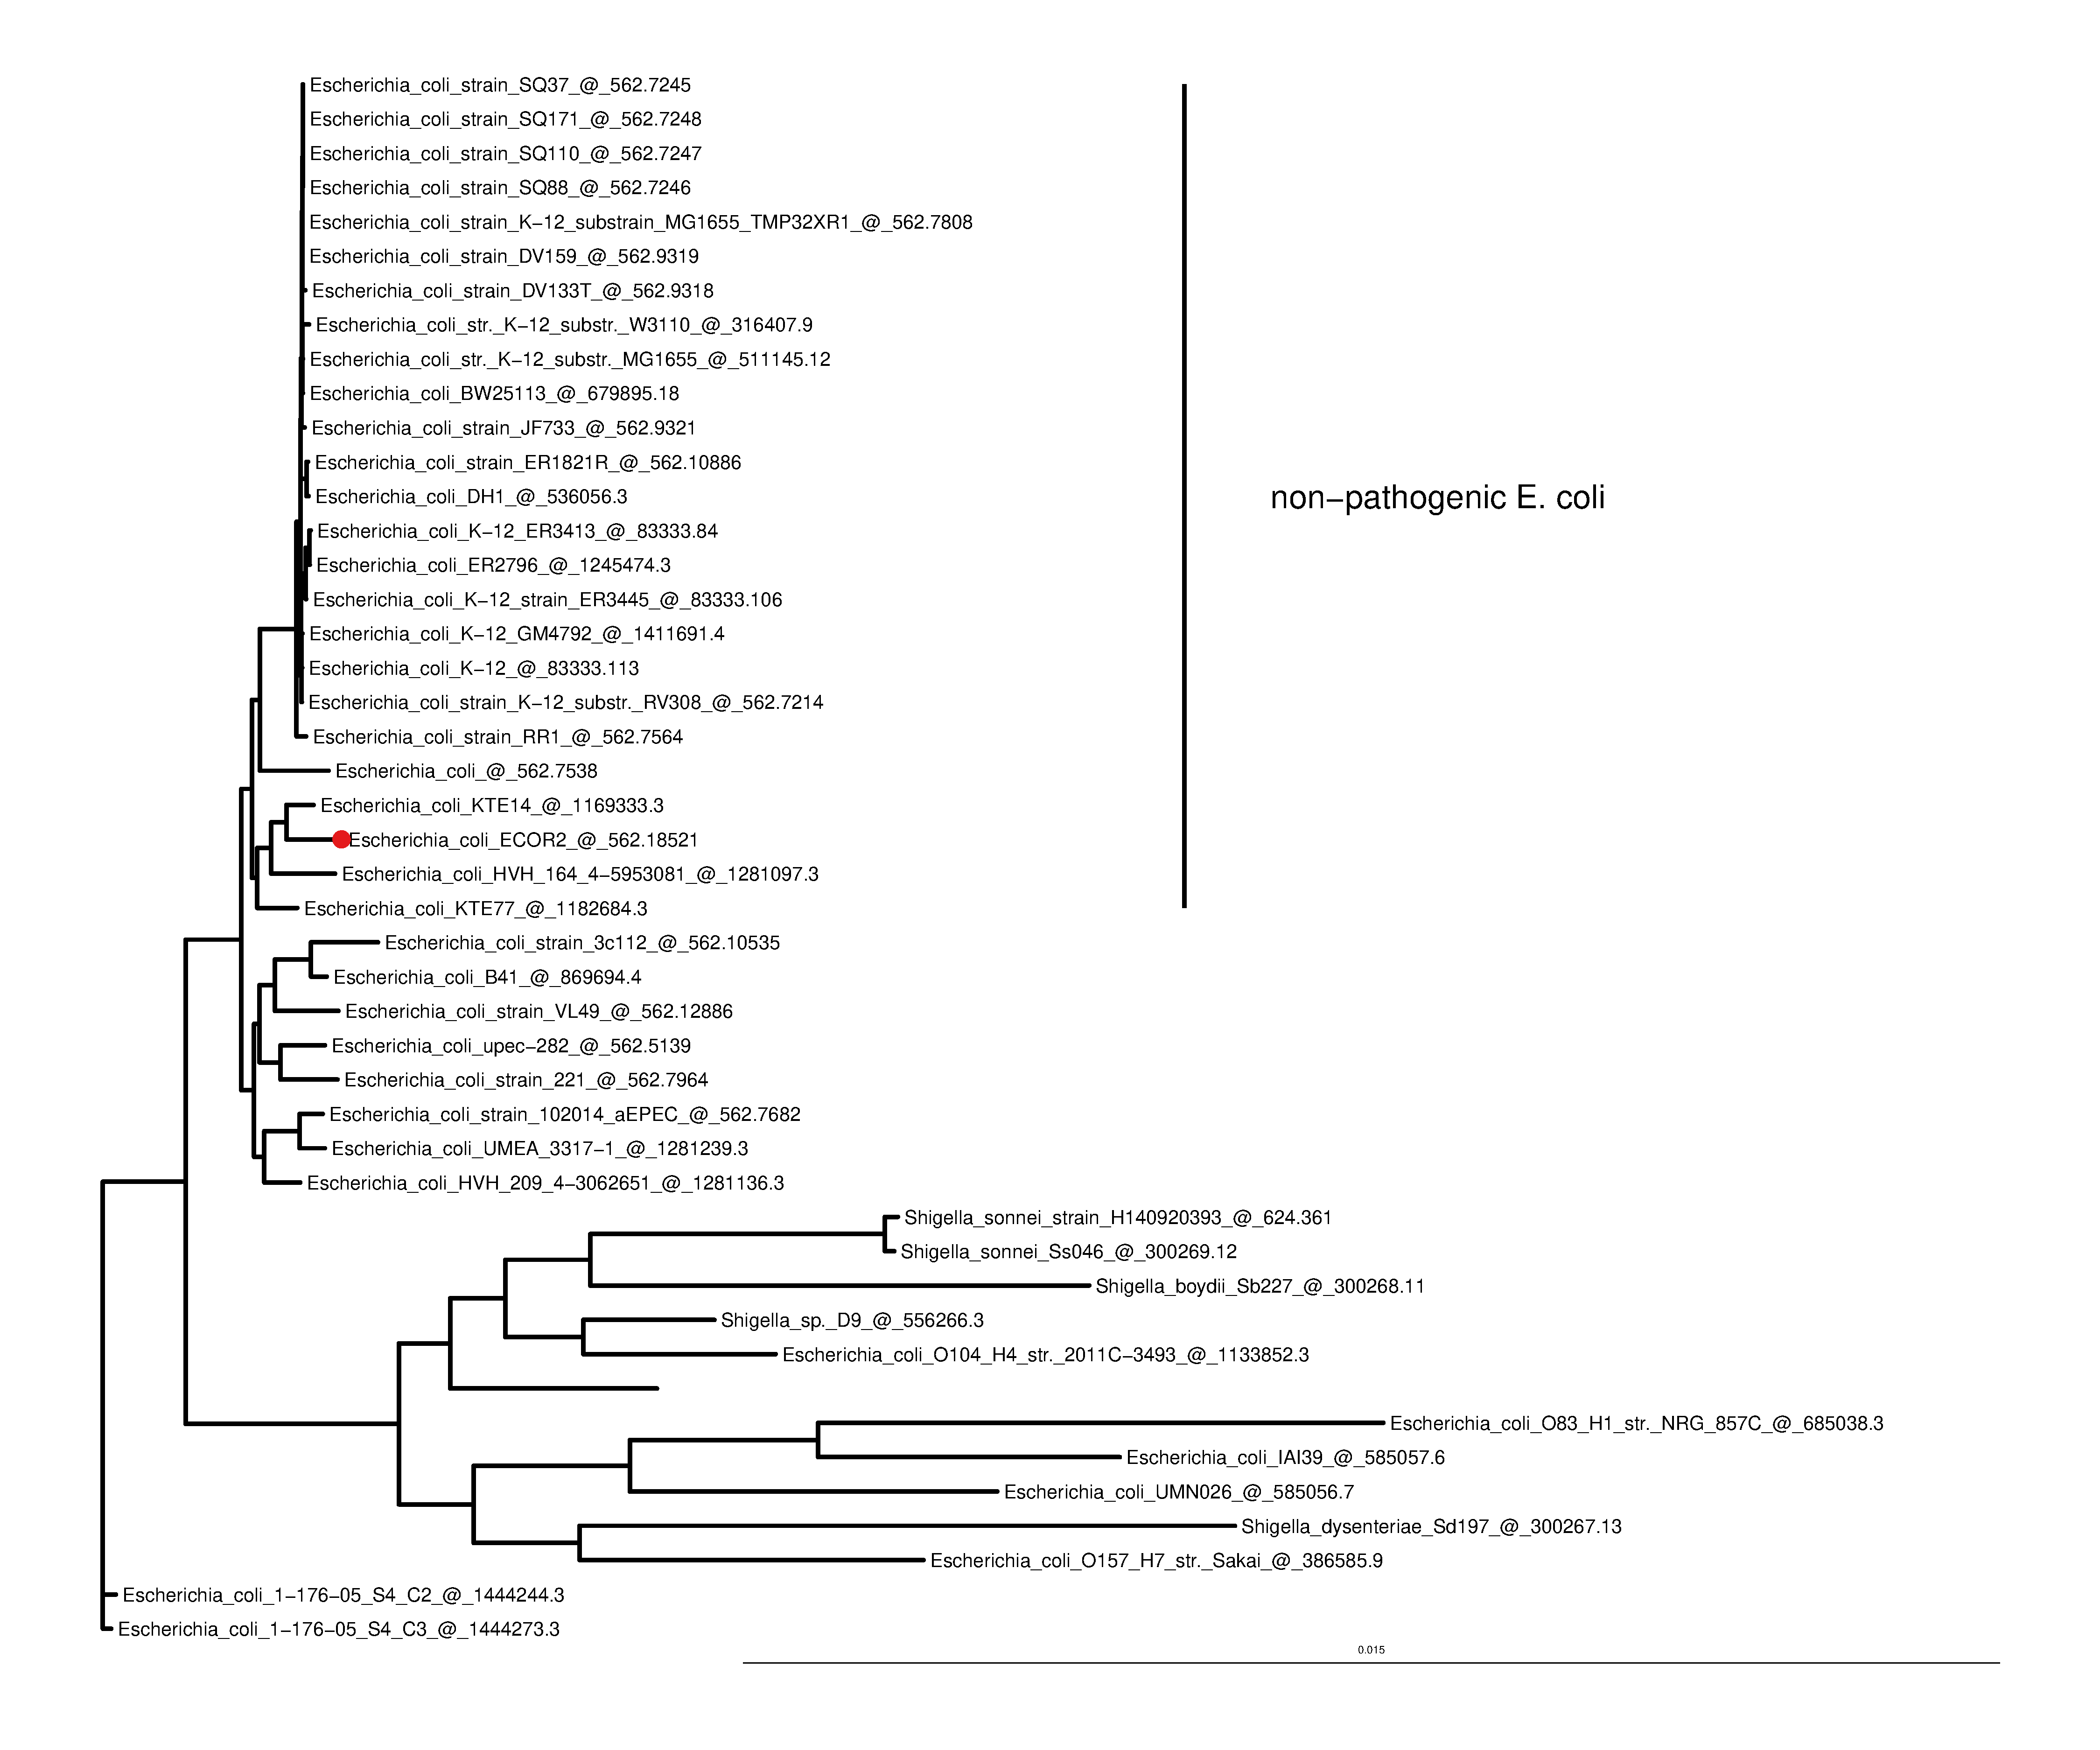
\includegraphics[width=0.9\linewidth]{./figures/figure1/sfigure1-2_tree.pdf}
 \caption*{\textbf{Figure 1 - Supplement 2. } Phylogenetic tree based on maximum liklihood genomic distance among \textit{E. coli} str. ECOR2 \citep{Ochman:1984}, the strain used in the HIO colonization experiments, closely related \textit{E. coli} isolates available on the PATRIC \citep{Wattam:2017} database, and pathogenic type strains from the genera \textit{Esherichia}, \textit{Shigella}, and \textit{Salmonella}. A PATRIC genome reference number follows name of each taxa.}
\label{fig:fullwidth}
\end{fullwidth}
\end{figure}
\bibliography{bibliography.bib}
\end{document}